%%%%%%%%%%%%%%%%%%%%% introduction.tex %%%%%%%%%%%%%%%%%%%%%%%%%%%%%%%%%
%
% Introduction chapter
%
%%%%%%%%%%%%%%%%%%%%%%%% Springer-Verlag %%%%%%%%%%%%%%%%%%%%%%%%%%

\chapter{Conteúdo}
\label{cont}

\section{Introducão}
\label{introduction} % Always give a unique label
% use \chaptermark{}
% to alter or adjust the chapter heading in the running head

Programação em lógica com restrições é uma junção de dois paradigmas: solução de restrições e programação em lógica. Esta combinação permite uma concepção mais expressiva e flexível — e em alguns casos mais eficiente - de problemas lógicos.

\subsection{Motivação}
\label{sec:1}
% Always give a unique label
% and use \ref{<label>} for cross-references
% and \cite{<label>} for bibliographic references
% use \sectionmark{}
% to alter or adjust the section heading in the running head
A motivação deste trabalho incidiu na compreensão de um paradigma de programação que já nos é familiar, envolvendo uma nova componente de restrições; resolver problemas lógicos com restrições de uma forma geral, tendo a possibilidade de os refinar e otimizar para uma solução particular.

\subsection{Objectivos}
\label{sec:2}
Resolver a versão original do jogo Turn12 recorrendo a restrições; gerar cubos com um número de dígitos variável, e avaliar se estes têm solução ou não segundo as restrições definidas.


\section{Descrição do problema}
\label{sec:3}
O problema centra-se num cubo em que cada face contém dígitos numerados de 3 a 9, aleatoriamente. Na junção das arestas de cada face, a soma dos dois dígitos que se encontram deverá ser igual a 12.

A solução original (Fig. \ref{fig:1}) com 24 dígitos por face é única.

Na geração de problemas, a resolução que apresentamos contempla dígitos ilimitados, e uma vez que não existe qualquer padrão associado à sequência de dígitos no problema original, estes são gerados aleatoriamente.

No entanto, para garantir a unicidade de solução, em valores demasiado elevados (superiores a 60 por face), as limitações de computação começaram-se a sentir e torna-se improvável gerar uma solução única em tempo útil.

%Figura cubo
\begin{figure}[H]
\begin{center}
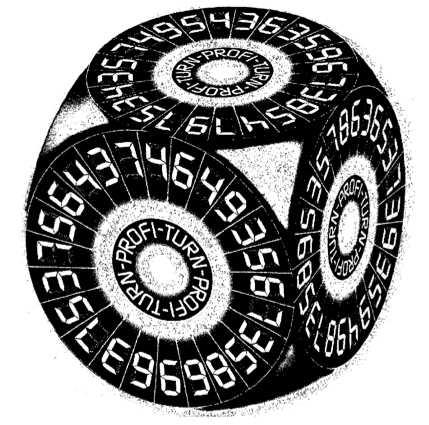
\includegraphics[scale=0.4]{turn12.png}
\caption{Problema original, com os pontos de contacto visíveis assinalados}
\label{fig:1}
\end{center}
\end{figure}



\section{Ficheiros de Dados}
\label{data:1}

Os ficheiros de dados são simples ficheiros de texto (\textit{.txt}), contendo em cada linha os dígitos de cada face.
As faces encontram-se pela seguinte ordem: Topo, Baixo, Frente, Trás, Esquerda e por fim Direita.

De seguida encontra-se um exemplo deste ficheiro com os valores do problema original:

\begin{f_exemplo}[H]
\begin{verbatim}

356735869637537564374649
343574954363596738547975
353748635975458485676439
349576573795398457964379
357863653739359498735895
348765738453874583769785
\end{verbatim}
\caption{Problema original do turn12, com 24 dígitos por face:}
\end{f_exemplo}



\section{Variáveis de Decisão}
\label{restr:1}

As variáveis de decisão usadas na solução foram as rotações que podiam ser feitas em cada face do cubo.\\
Estas rotações têm um domínio compreendido entre 1 e o número de dígitos de cada face.

\section{Restrições}
\label{restr:2}

Independentemente do número de dígitos em cada face, verificou-se que as restrições seriam sempre as mesmas: a soma dos dígitos no ponto de contacto entre duas faces tem de ser 12.\\

Na implementação foi utilizado no \textit{SICStus Prolog} a biblioteca de restrições para o conjunto dos domínios finitos \textit{clp(FD)}, onde foram definidas variáveis que seriam preenchidas com os valores dos pontos de contacto tendo em conta a rotação aplicada sobre cada face, e restringidas de forma a que a soma dos mesmos seja obrigatoriamente 12.

\section{Função de Avaliação}
\label{restr:3}

Os predicados de avaliação chamam-se \textit{turn12}. Foram implementados três com o mesmo nome na solução, mas o principal aceita como parâmetros de entrada as 6 faces do cubo, que deverão ser cada um uma lista numérica de dígitos. Se for encontrada uma solução, são definidos como parâmetros de saída as rotações respectivas de cada face. São também definidos e agrupados 4 a 4 os valores da solução. Este predicado tem como objectivo apenas retornar a primeira solução encontrada.\\
O segundo predicado, com o mesmo nome, tem como parâmetro de entrada a localização do ficheiro com a informação de cada face, e só termina até imprimir todas as soluções do problema.
Por fim, existe ainda um último predicado que não aceita qualquer parâmetro, e que chama o predicado anteriormente descrito, com um ficheiro numa localização predefinida.


\section{Estratégia de Pesquisa}
\label{rest:4}

A estratégia de pesquisa baseia-se na rotação de cada face até encontrar uma solução.
De forma a optimizar a resolução do problema, o algoritmo começa apenas com duas faces, e tenta encontrar através do predicado de etiquetagem \textit{labeling} uma rotação que consiga somar o valor 12 nos seus pontos de contactoo.
Quando encontrada, é passada para outra face do cubo, e com recurso a outro predicado de etiquetagem é tentado encontrar uma rotação para esta última que consiga satisfazer as mesmas restrições para os pontos de contacto em comum com as duas faces anteriores. É seguida sempre a mesma estratégia para as restantes faces, fazendo com que a complexidade algorítmica seja sempre a menor possível.
A razão para a utilização de vários predicados de etiquetagem deve-se ao facto de ser utilizado um predicado auxiliar (\textit{shifted\_face}), que preenche as variáveis utilizadas para testar as restrições com base na rotação correspondente. 
Verificou-se que, quando utilizado um único predicado para o mesmo efeito, o \textit{shifted\_face} era chamado desnecessariamente mesmo para as faces em que a rotação se mantinha igual e que não tinham originado a falha.
Após isolados, o predicado só passou a ser chamado para a face do respectivo labeling, e evitando um varrimento contínuo e dispendioso nas várias listas de dígitos de cada face.

\section{Visualização da Solução}
\label{rest:5}

A visualização da solução é feita através do predicado \textit{project\_cube}.
Este predicado faz uma projecção (Fig. \ref{fig:2}) do cubo de 3 dimensões em 2, e tem como parâmetros de entrada os valores da solução encontrada pelo algorítmo de procura. Estes parâmetros são passados em grupos de 4, representando os pontos de contacto de cada face pela seguinte ordem: ponto superior, direito, inferior e esquerdo. 
A ordem de passagem das faces é : Topo,Traseira, Direita, Esquerda, Dianteira, Inferior.

\begin{figure}[H]
\begin{center}
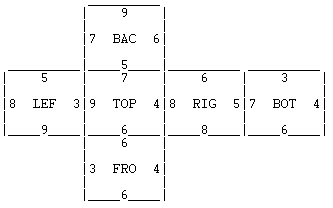
\includegraphics[scale=0.6]{resol.png}
\caption{Impressão da solução do problema original do turn12.}
\label{fig:2}
\end{center}
\end{figure}

Adicionalmente, foi desenvolvido o predicado \textit{print\_rots}, que imprime o número de rotações (Fig. \ref{fig:3})  que devem ser dadas em cada face sobre o problema original para chegar à solução, no sentido contrário ao dos ponteiro do relógio.

\begin{figure}[H]
\begin{center}
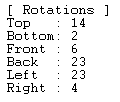
\includegraphics[scale=0.6]{rots.png}
\caption{Impressão das rotações do problema original do turn12.}
\label{fig:3}
\end{center}
\end{figure}


\section{Resultados}
\label{rest:6}

De seguida seguem-se dois exemplos da resolução de dois problemas com complexidades diferentes, gerados com o predicado \textit{turn12gen}

\begin{f_exemplo}[H]
\begin{verbatim}

8987698939348595456596537597964569768569756345737893
6756434375953493785343639458956939579893487543689353
3579793975458794354537534574645348648939348956983756
6789345463497649386734675747959348987858395394783478
4636795348358376783754934938935675854758379538676936
6456984789496935693937974554589635464347893474635735
\end{verbatim}
\caption{Problema com 52 dígitos por face:}
\end{f_exemplo}

\begin{figure}[H]
\begin{center}
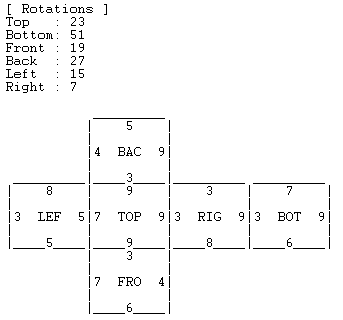
\includegraphics[scale=0.7]{ex1.png}
\caption{Solução do problema com 52 dígitos por face}
\label{fig:4}
\end{center}
\end{figure}

\begin{f_exemplo}[H]
\begin{verbatim}

894896346958797867878397593785997678947876483959373486864543438685698676
739475798946785793456537485839735954538537834873597678963893563438758346
876768685479345693587896839654685468943463769386734938644896978963478579
467998968397969378534737893478583896345647846478475486739653976367948939
469893649494653679565694856947898675395494956976355856784965975784895785
784837634596534396493678394685453865348743489746597473438967439397839853
\end{verbatim}
\caption{Problema com 72 dígitos por face:}
\end{f_exemplo}

\begin{figure}[H]
\begin{center}
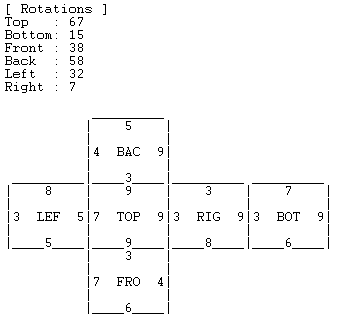
\includegraphics[scale=0.7]{ex2.png}
\caption{Solução do problema com 72 dígitos por face}
\label{fig:4}
\end{center}
\end{figure}



%
